\section{Методи та результати}

Для проведення дослідження використовувався набір даних Spotify Tracks Dataset у форматі CSV. Аналіз виконувався мовою Python із використанням бібліотек pandas, matplotlib, seaborn та scikit-learn.

На початковому етапі було виконано попередню обробку даних. Було перевірено наявність пропущених значень, виконано очищення набору даних та підготовлено числові ознаки для подальшого аналізу.

\subsection{Описовий аналіз даних}

Було досліджено розподіли основних аудіофіч, зокрема energy, danceability, loudness, acousticness та popularity. Аналіз показав, що більшість композицій мають середній або високий рівень енергійності та танцювальності.

\begin{figure}[H]
  \centering
  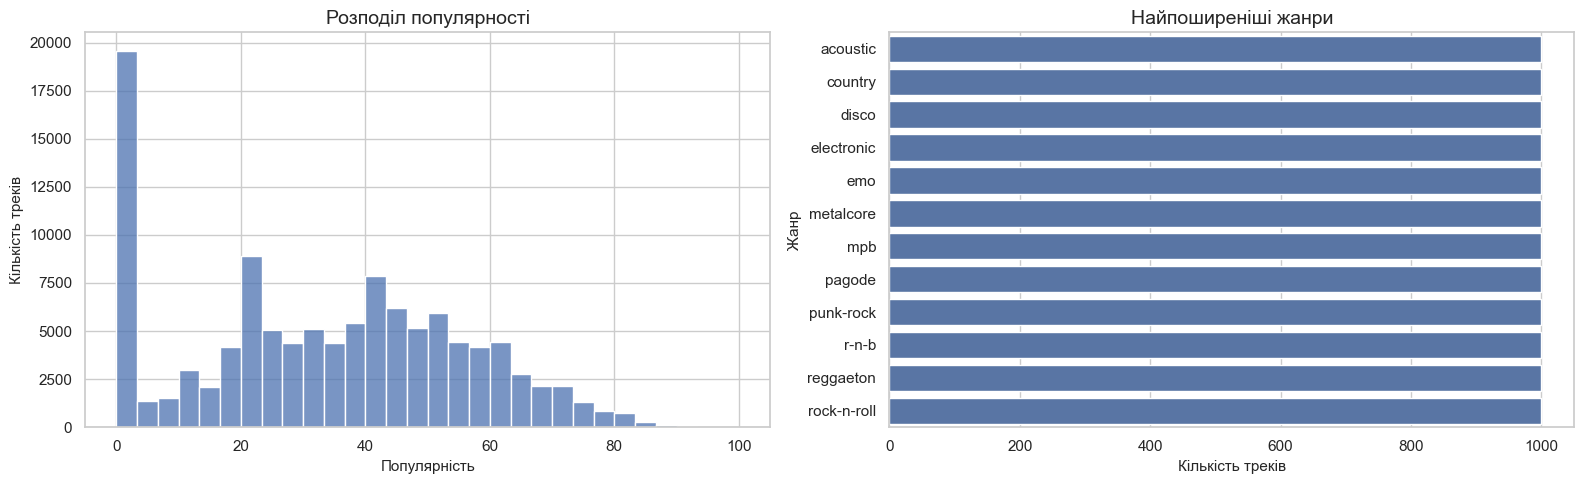
\includegraphics[width=\linewidth]{images/distributions.png}
  \caption{Розподіли основних аудіофіч}
  \label{fig:distributions}
\end{figure}

\subsection{Кореляційний аналіз}

Наступним етапом було виконано кореляційний аналіз між аудіофічами. Найбільш помітні залежності спостерігалися між energy та loudness, а також між acousticness та energy.

\begin{figure}[H]
  \centering
  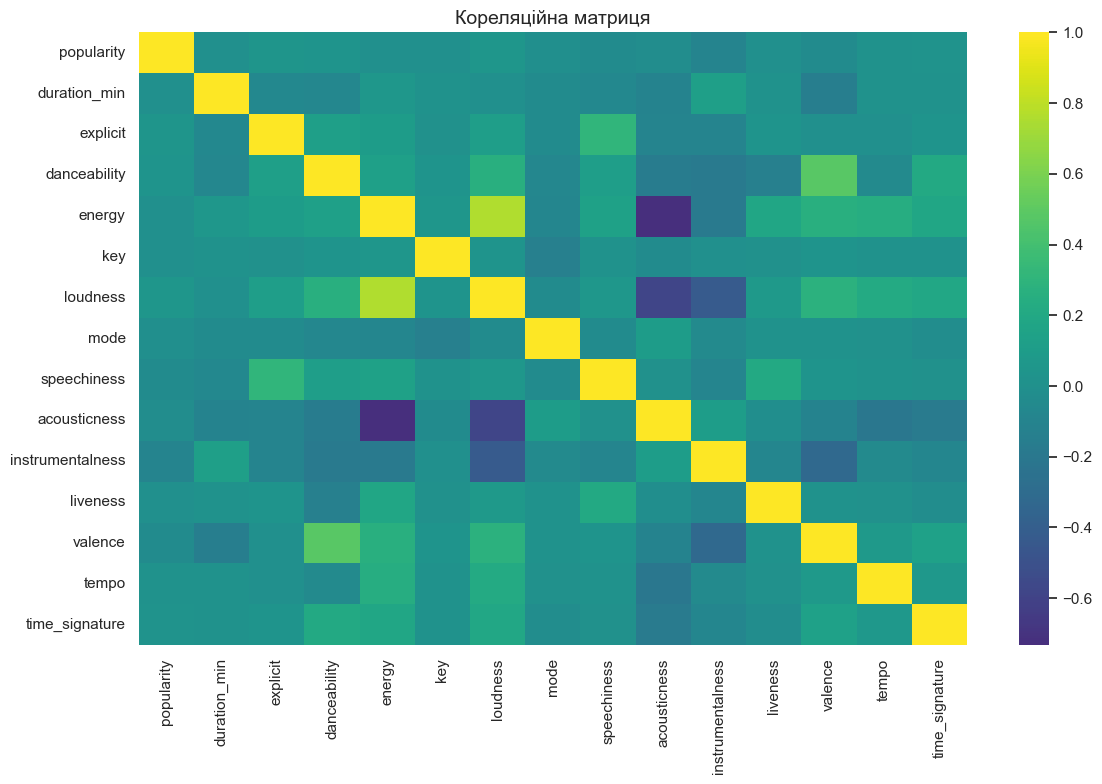
\includegraphics[width=\linewidth]{images/correlation_matrix.png}
  \caption{Матриця кореляцій аудіофіч}
  \label{fig:correlation}
\end{figure}

Кореляційна матриця дозволила виявити як позитивні, так і негативні взаємозв'язки між характеристиками композицій.

\subsection{Кластеризація треків}

Для групування композицій було використано алгоритм KMeans. Перед побудовою моделі було виконано нормалізацію ознак. Кількість кластерів обиралася на основі методу ліктя та silhouette score.

\begin{figure}[H]
  \centering
  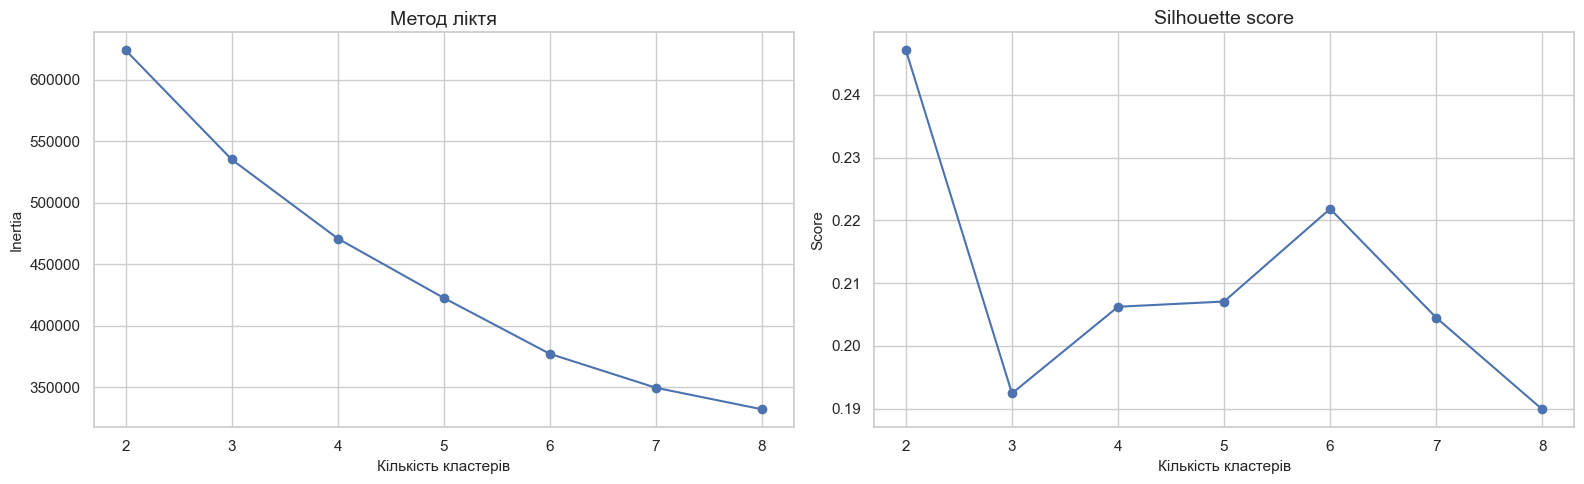
\includegraphics[width=\linewidth]{images/elbow_method.png}
  \caption{Вибір кількості кластерів методом ліктя}
  \label{fig:elbow}
\end{figure}

Після визначення оптимальної кількості кластерів було побудовано фінальну модель кластеризації.

\begin{figure}[H]
  \centering
  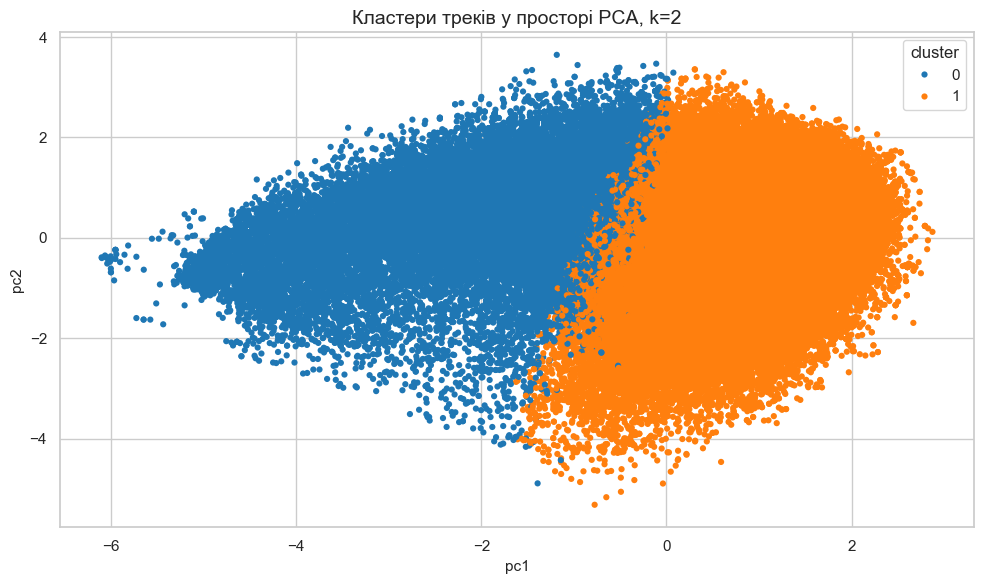
\includegraphics[width=\linewidth]{images/pca_clusters.png}
  \caption{Візуалізація кластерів після PCA}
  \label{fig:pca}
\end{figure}

Результати показали, що композиції формують декілька відносно стабільних груп із подібними характеристиками.

\subsection{Класифікація популярності треків}

Для прогнозування популярності треків використовувалися моделі Logistic Regression та Random Forest. Цільова змінна формувалася шляхом поділу треків на популярні та непопулярні відносно медіанного значення popularity.

Random Forest продемонстрував кращу якість класифікації порівняно з Logistic Regression, що свідчить про наявність нелінійних залежностей у даних.

\begin{figure}[H]
  \centering
  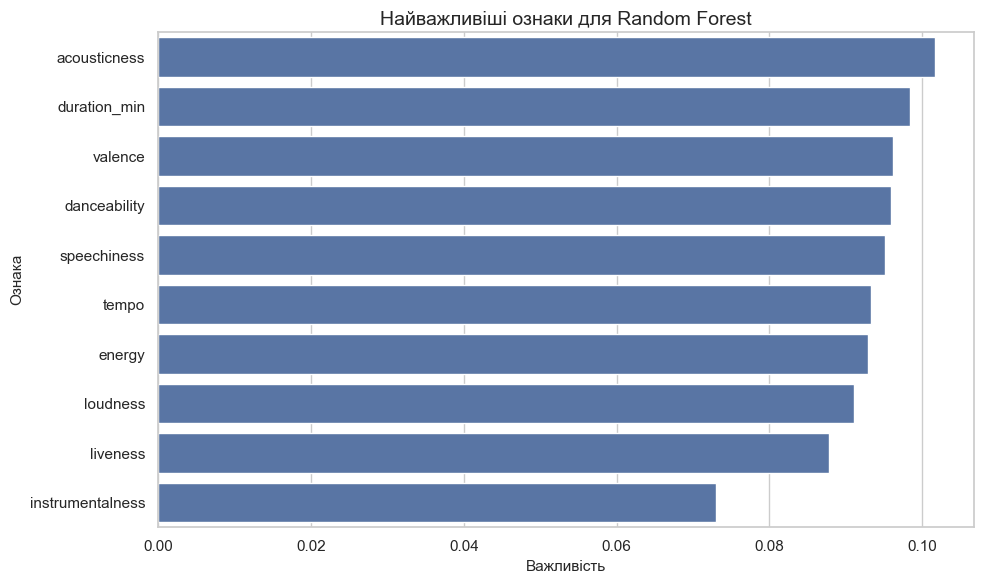
\includegraphics[width=\linewidth]{images/feature_importance.png}
  \caption{Важливість ознак у моделі Random Forest}
  \label{fig:importance}
\end{figure}

Найбільш значущими ознаками для прогнозування популярності виявилися energy, danceability, loudness та valence.

\begin{figure}[H]
  \centering
  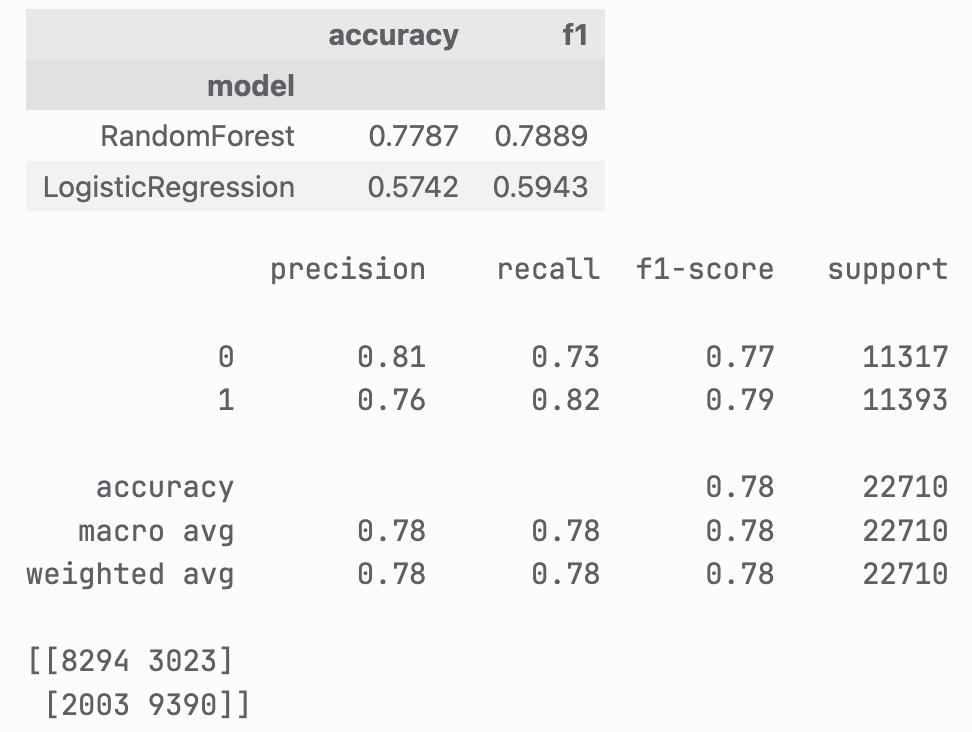
\includegraphics[width=\linewidth]{images/confusion_matrix.png}
  \caption{Матриця помилок моделей Random Forest та Logistic Regression}
  \label{fig:confusion}
\end{figure}

Отримані результати підтверджують ефективність використання методів інтелектуального аналізу даних для дослідження музичних композицій та прогнозування їх популярності.
